\begin{figure*}[!htb]
    \centering
    \subfigure[MI by Decision]{
    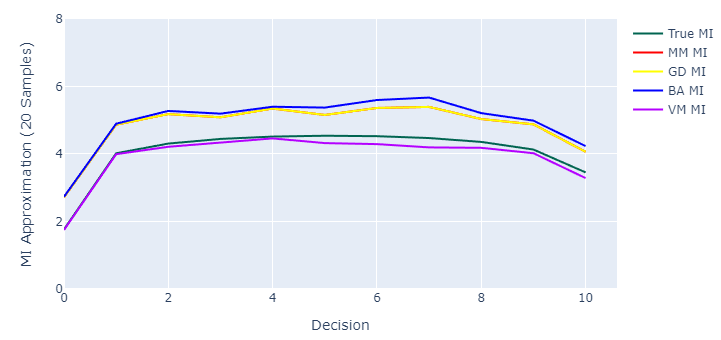
\includegraphics[width=.48\textwidth]{ABMI20.png}
    }
    \subfigure[Gradient Step Convergence]{
    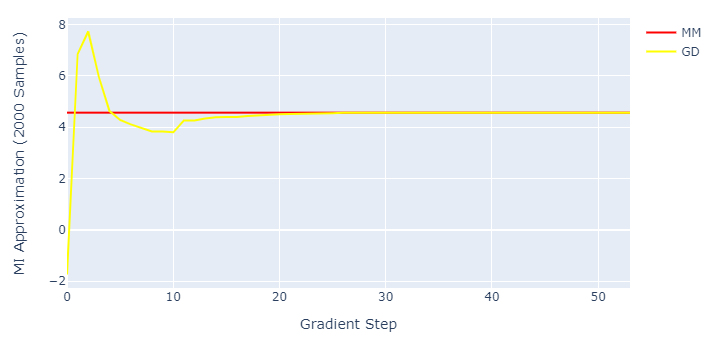
\includegraphics[width=.47\textwidth]{ABGDStep.png}
    }
    \caption{\textbf{A/B Test} for $11$ decisions of assigning $10$ participants to $2$ groups. Because the method is Gaussian linear, each model converges to the true Mutual Information. (a) $20$ samples were used to compute the mutual Information for each decision (b) This plot shows the convergence of the Gradient Descent approach approximation with respect to the number of Gradient Steps. Notice that the Gradient step converges to the Moment Matching Solution but takes $~50$ steps. The Moment Matching reaches this end convergence immediately without needing to do multiple evaluations.}
    \label{fig:ABDGStep}
    \end{figure*}
    
    We consider the classical A/B test with a Gaussian linear model. The experiment 
    in this case is where $D$ participants are chosen to be split into two 
    groups, $A$ and $B$. The design is the choice of the group size, $d_A$ for 
    group $A$ and $d_B=N-d_A$ for group $B$. Each participant then has a measured 
    continuous response $y$. The Bayesian model is a Gaussian linear as follows.
    \begin{equation}
    x\sim N(0,\Sigma_x)\hspace{2em} y|x,d \sim N(D_dx,I)\hspace{2em}\Sigma_x = \begin{bmatrix}
    10^2 & 0 \\
    0 & 1.82^2
    \end{bmatrix}
    \end{equation}
    where $D_d$ is the design matrix of size $D\times 2$ with the first $d_A$ rows 
    as $(1,0)$ and the remaining as $(0,1)$ to signify group assignments. For this 
    experiment, we will us $D=10$ participants.\\
    For variational distribution, we assumed linear multivariate gaussians from 
    the Exponential Family for both the marginal and likelihood. To evaluate each 
    approximation, $N$ samples are drawn from the prior and then the posterior 
    as $x_n\sim p(x)$ and $y_n\sim p(y|x=x_n)$.\\
    
    Figure \ref{fig:ABDGStep} shows the evaluations of Moment Matching, Gradient 
    Descent, Variational Posterior, and Variational Marginal to the true Mutual 
    Information $N=20$ Sample Points. Notice, the Moment Matching and Gradient 
    Descent Approach both match for each decision evaluation as expeceted. In 
    Figure  \ref{fig:ABDGStep}, we compare the Mutual Information evaluation of 
    Moment Matching to that of Gradient Descent with respect to gradient steps. 
    Notice that Gradient Descent approaches the Moment match solution but take 
    approximately K step before it has leveled out.\\
    
    Another important property to observe from the Figure \ref{fig:ABDGStep} is 
    that the theoretical bound have been swapped for Varaitional Posterior and 
    Variational Marginal distributions, that is Variational Marginal should be 
    an upper bound but is a lower bound and vice-versa. This is due to a bias 
    introduced from finite sample plug in estimators. It is easily shown 
    that $\E[\hat{\Sigma}]=\frac{n+1}{n-1}\Sigma$. So in this case where our 
    variational distributions are the same family as the target distributions 
    (Gaussian), the error bound from Gibbs' inequality is less than that of the 
    introduced bias and the bound swaps. For examples where the target distribution 
    is not a Gaussian, the bias tends to be negligible compared to the approximation 
    bound.\\
    
    For further analysis, Figure \ref{fig:ABConvergence}, the convergence rate and 
    time of each method is shown for the decision with the maximum Mutual 
    Information ($d=5$) with respect to the number of samples taken. We notice after 
    a few hundred samples, all of the methods have converged to the true Mutual 
    Information. We also see that for computation time, every method is orders of 
    magnitude faster than that of the Gradient Descent. We will see that as the 
    dimensionality of the problem increases, the speed of Moment Matching will be 
    highlighted in comparison to Variational Marginal and Variational Posterior.
    
    \begin{figure*}[!htb]
    \centering
    \subfigure[MI Convergence]{
    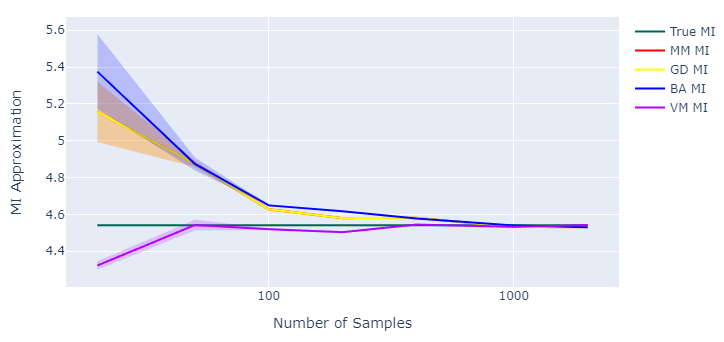
\includegraphics[width=.48\textwidth]{ABConverge.png}
    }
    \subfigure[Computation Time]{
    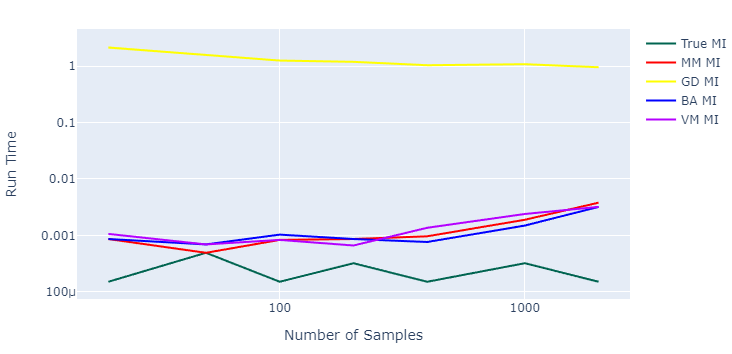
\includegraphics[width=.47\textwidth]{ABTime.png}
    }
    \caption{\textbf{A/B Test Mutual Information Estimation} for $11$ decisions of assigning $10$ participants to $2$ groups. Because the method is Gaussian linear, each model converges to the true Mutual Information. (a) The convergence of MI with respect to the number of samples drawn is plotted for the maximum MI decision ($d=5$) (b) The run time of each method is plotted for the number of samples for the maximum MI decision ($d=5$). Note that Moment Matching and Gradient Descent Match in approximation Value however Moment matching save orders of magnitude in computation time. }
    \label{fig:ABConvergence}
    \end{figure*}